
\documentclass[tikz,border=6mm]{standalone}
\usepackage[T1]{fontenc}
\usepackage[utf8]{inputenc}
\usepackage{lmodern}
\usepackage{amsmath}
\usepackage{xcolor}
\usetikzlibrary{arrows.meta,calc,positioning}

\definecolor{TitleBlue}{HTML}{1D2C57}
\definecolor{NvidiaGreen}{HTML}{76B900}
\definecolor{LoadA}{HTML}{D9E5F7}
\definecolor{LoadB}{HTML}{DCEAD3}
\definecolor{Compute}{HTML}{F7DDA8}
\definecolor{Warmup}{HTML}{EEEAF4}
\definecolor{Startup}{HTML}{F8F1DE}
\definecolor{Steady}{HTML}{E8EEF8}
\definecolor{SoftGray}{HTML}{F5F6F8}
\definecolor{Grid}{HTML}{989898}
\definecolor{Dark}{HTML}{222222}

\tikzset{
  title/.style={font=\sffamily\bfseries\LARGE,text=TitleBlue,align=center},
  subtitle/.style={font=\sffamily\large,text=Dark,align=center},
  lane/.style={font=\sffamily\bfseries\large,text=Dark,anchor=east},
  tick/.style={font=\sffamily\large,text=Dark},
  loadA/.style={draw=TitleBlue!90!black,rounded corners=2pt,line width=1.0pt,fill=LoadA},
  loadB/.style={draw=NvidiaGreen!65!black,rounded corners=2pt,line width=1.0pt,fill=LoadB},
  comp/.style={draw=brown!55!black,rounded corners=2pt,line width=1.0pt,fill=Compute},
  note/.style={draw=Grid,rounded corners=2pt,line width=0.9pt,fill=SoftGray,font=\sffamily\large,text=Dark,align=left},
}

\begin{document}
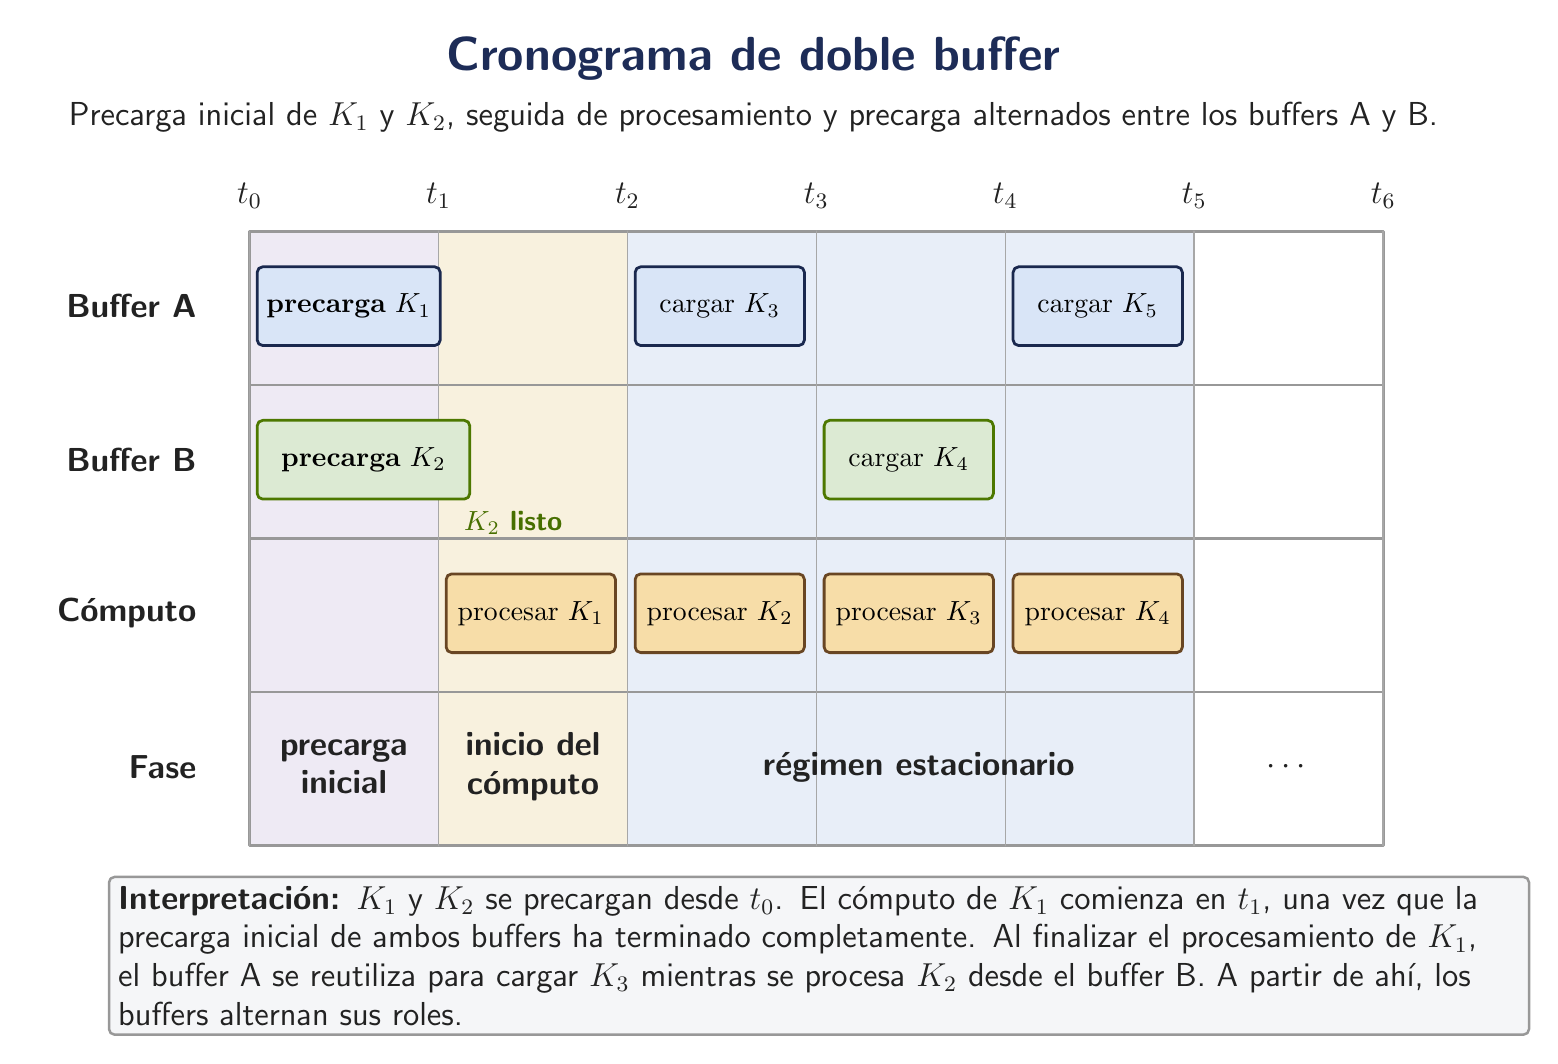
\begin{tikzpicture}[x=1cm,y=1cm,line cap=round,line join=round]

% Title
\node[title,text width=18.2cm] at (9.5,12.1)
  {Cronograma de doble buffer};
\node[subtitle,text width=18cm] at (9.5,11.35)
  {Precarga inicial de $K_1$ y $K_2$, seguida de procesamiento y precarga alternados entre los buffers A y B.};

% Geometry
\def\xL{3.10}
\def\xR{17.50}
\def\yT{9.90}
\def\yB{2.10}

% Main time marks:
% t0=3.10, t1=5.50, t2=7.90, t3=10.30, t4=12.70, t5=15.10, t6=17.50

% Phase backgrounds: all shading stops exactly at t5
\fill[Warmup] (\xL,\yB) rectangle (5.50,\yT);
\fill[Startup] (5.50,\yB) rectangle (7.90,\yT);
\fill[Steady]  (7.90,\yB) rectangle (15.10,\yT);

% Frame
\draw[Grid,line width=0.9pt] (\xL,\yB) rectangle (\xR,\yT);
\foreach \y in {7.95,6.00,4.05}{
  \draw[Grid,line width=0.85pt] (\xL,\y) -- (\xR,\y);
}
\foreach \x/\lab in {3.10/$t_0$,5.50/$t_1$,7.90/$t_2$,10.30/$t_3$,12.70/$t_4$,15.10/$t_5$,17.50/$t_6$}{
  \draw[Grid!85,line width=0.65pt] (\x,\yB) -- (\x,\yT);
  \node[tick] at (\x,10.35) {\lab};
}

% Lane labels
\node[lane] at (2.55,8.95) {Buffer A};
\node[lane] at (2.55,7.00) {Buffer B};
\node[lane] at (2.55,5.05) {Cómputo};
\node[lane] at (2.55,3.10) {Fase};

% Top labels: only K2 marker remains, no K1/start-compute label
\node[font=\sffamily\bfseries\normalsize,text=NvidiaGreen!60!black] at (6.45,6.20)
  {$K_2$ listo};

% Buffer A
\node[loadA,anchor=west,minimum width=2.15cm,minimum height=1.00cm] at (3.18,8.95) {\textbf{precarga} $K_1$};
\node[loadA,anchor=west,minimum width=2.15cm,minimum height=1.00cm] at (7.98,8.95) {cargar $K_3$};
\node[loadA,anchor=west,minimum width=2.15cm,minimum height=1.00cm] at (12.78,8.95) {cargar $K_5$};

% Buffer B
\node[loadB,anchor=west,minimum width=2.70cm,minimum height=1.00cm] at (3.18,7.00) {\textbf{precarga} $K_2$};
\node[loadB,anchor=west,minimum width=2.15cm,minimum height=1.00cm] at (10.38,7.00) {cargar $K_4$};

% Compute row
\node[comp,anchor=west,minimum width=2.15cm,minimum height=1.00cm] at (5.58,5.05) {procesar $K_1$};
\node[comp,anchor=west,minimum width=2.15cm,minimum height=1.00cm] at (7.98,5.05) {procesar $K_2$};
\node[comp,anchor=west,minimum width=2.15cm,minimum height=1.00cm] at (10.38,5.05) {procesar $K_3$};
\node[comp,anchor=west,minimum width=2.15cm,minimum height=1.00cm] at (12.78,5.05) {procesar $K_4$};

% Phase row labels only (no arrows)
\node[font=\sffamily\bfseries\large,text=Dark,align=center] at (4.30,3.10) {precarga\\inicial};
\node[font=\sffamily\bfseries\large,text=Dark,align=center] at (6.70,3.10) {inicio del\\cómputo};
\node[font=\sffamily\bfseries\large,text=Dark,align=center] at (11.60,3.10) {régimen estacionario};
\node[font=\sffamily\large,text=Dark] at (16.30,3.10) {$\cdots$};

% Interpretation box
\node[note,text width=17.8cm,anchor=west] at (1.30,0.70) {
\textbf{Interpretación:} $K_1$ y $K_2$ se precargan desde $t_0$. El cómputo de $K_1$ comienza en $t_1$, una vez que la precarga inicial de ambos buffers ha terminado completamente. Al finalizar el procesamiento de $K_1$, el buffer A se reutiliza para cargar $K_3$ mientras se procesa $K_2$ desde el buffer B. A partir de ahí, los buffers alternan sus roles.
};

\end{tikzpicture}
\end{document}
